\begin{figure*}[h!t]
 \begin{center} 
  \begin{tabular}{ll}
\begin{tabular}{|l|l|l|l|l|}
\hline
\multicolumn{1}{|r|}{\textit{\textbf{Low Input}}} & fact(20) in $ns$           & fib(20) in $ns$           & tailfact(20) in $ns$      & evenodd(256) in $\mu s$           \\ \hline
\textbf{IFO}                                      & $204.84 \pm 2.35$   & $35.50 \pm 0.47$   & $49.52 \pm 0.72$  & $32.95 \pm 0.09$    \\ \hline
\textbf{Java}                                     & $147.95 \pm 0.65$   & $22.50 \pm 0.06$   & $18.18 \pm 0.19$  & $30.93 \pm 0.12$   \\ \hline
\textbf{Java (T)}                                 & $1280.23 \pm 20.99$ & $502.35 \pm 9.42$ & $139.39 \pm 1.79$ & $474.41 \pm 6.29$ \\ \hline
\textbf{Scala}                                    & $130.46 \pm 0.40$    & $22.55 \pm 0.14$  & $15.94 \pm 0.05$  & $32.79 \pm 0.09$    \\ \hline
\textbf{Clojure}                                  & $573.95 \pm 3.41$   & $314.24 \pm 2.25$ & $205.21 \pm 0.35$ & $82.61 \pm 0.95$   \\ \hline
\end{tabular}
 &
\begin{tabular}{|l|l|l|}
\hline
\multicolumn{1}{|r|}{\textit{\textbf{\begin{tabular}[c]{@{}r@{}}High\\ Input\end{tabular}}}} & \begin{tabular}[c]{@{}l@{}}evenodd\\ (214748) in $\mu s$\end{tabular} & \begin{tabular}[c]{@{}l@{}}tailfact\\ (10000) in $\mu s$\end{tabular} \\ \hline
\textbf{IFO}                                                                                               & $152.47 \pm 0.43$     & $166.64 \pm 0.51$    \\ \hline
\textbf{Java}                                                                                              & $1060.35 \pm 14.52$ & $644.10 \pm 3.89$   \\ \hline
\textbf{Scala}                                                                                              & $1864.34 \pm 31.24$  & $1004.13 \pm 13.49$ \\ \hline
\textbf{Clojure}                                                                                           & $6533.14 \pm 92.65$ & N/A                       \\ \hline
\end{tabular}
\end{tabular}
  \begin{tabular}{ll}
  \begin{minipage}{8cm}{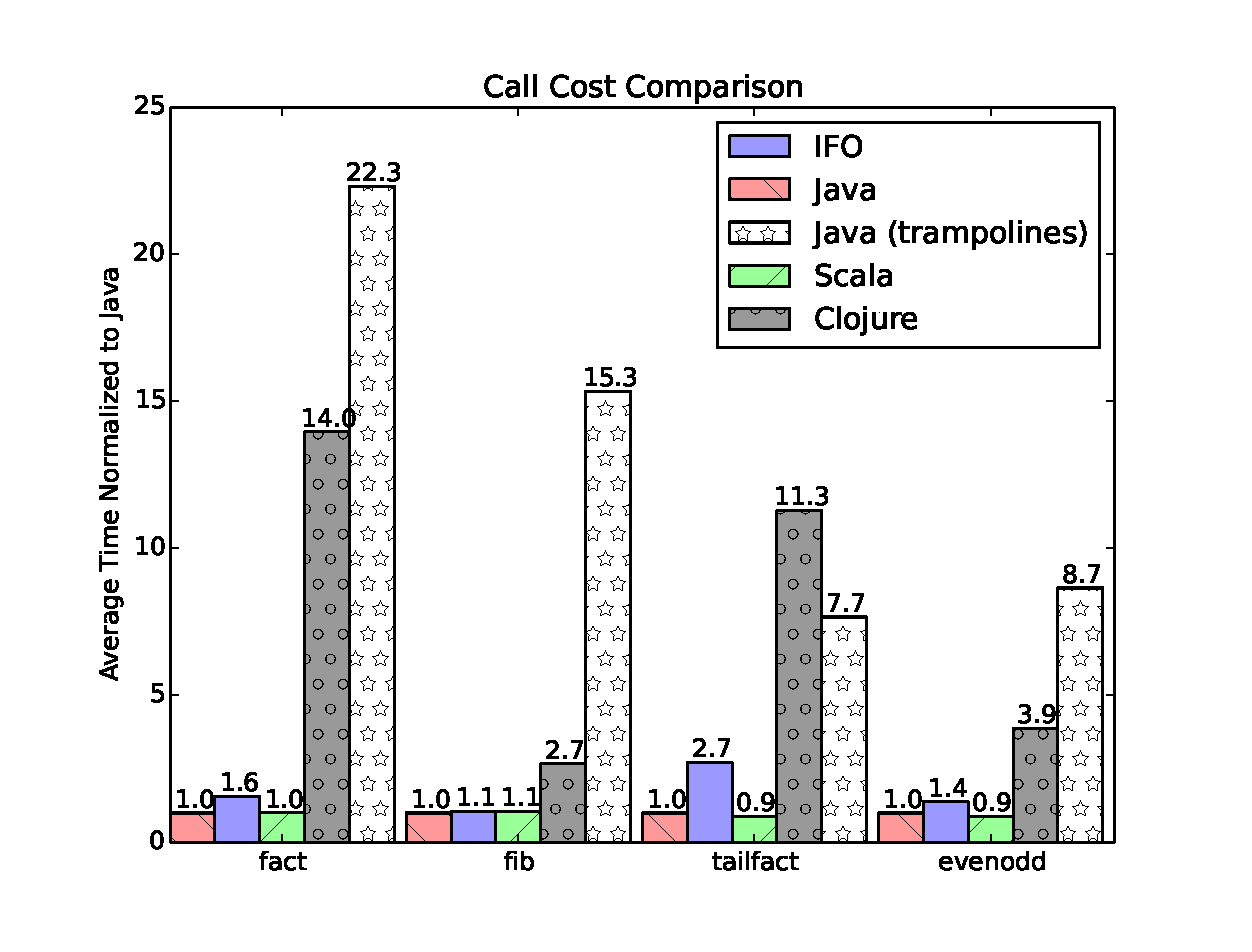
\includegraphics[width=8cm]{./src/img/low.eps}}\end{minipage} &
\begin{minipage}{8cm}{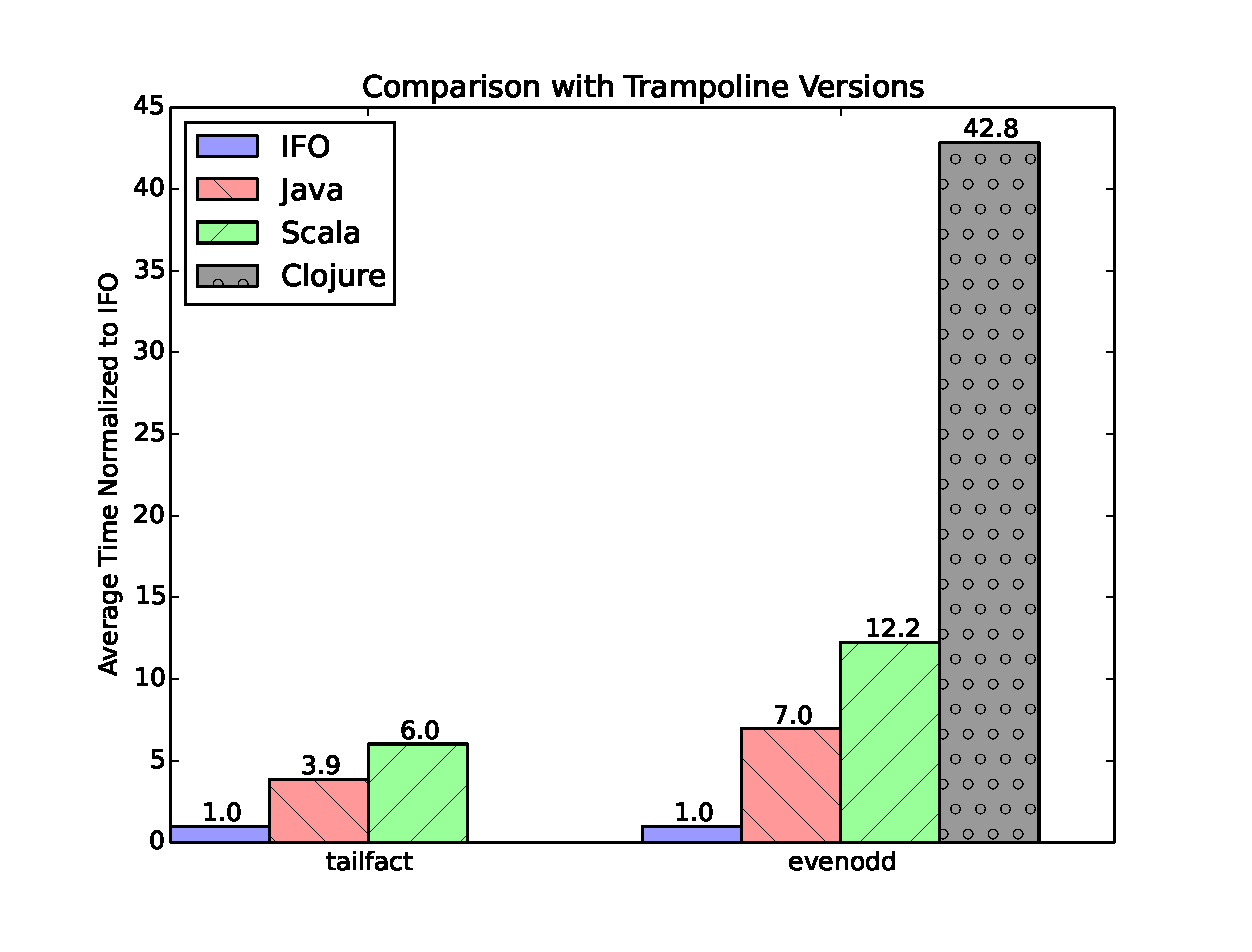
\includegraphics[width=8cm]{./src/img/high.eps}}\end{minipage}
\end{tabular}

\end{center}
\vspace{-20pt}
  \caption{The isolated call behavior experiments: the reported times are averages of 10 measured runs and corresponding standard deviations. The plots are normalized to Java's (left table and plot) and IFO's (right table and plot) results -- the lower, the faster.}

\label{fig:micro}
\end{figure*}

\begin{figure*}[h!t]
\vspace{10pt}
 \begin{center} 
\begin{tabular}{|l|l|l|l|l||l|l|}
\hline
\multicolumn{1}{|r|}{\textit{\textbf{Input length (time unit)}}} & 1000 ($\mu s$)                 & 3000 ($\mu s$)                  & 10000 ($\mu s$)                   & 100000 ($\mu s$)    & Objects (Min) & Objects (Max)               \\ \hline
\textbf{IFO}                                  & $5.10 \pm 0.10$   & $15.98 \pm 0.07$  & $77.81 \pm 0.83$   & $933.58 \pm 13.40$ &  5451 & 5451    \\ \hline
\textbf{Java (Trampoline-based)}                             & $7.03 \pm 0.130$ & $26.89 \pm 0.10$ & $102.98 \pm 2.36$ & $1099.80 \pm 15.46$ & 4665 & 104879\\ \hline
\textbf{Java (Method-based)}                             & $3.80 \pm 0.07$  & $11.61 \pm 0.10$  & $48.83 \pm 0.13$    & N/A  & 4128 & 4128                      \\ \hline
\textbf{Java (FAO-based)}                           & $6.37 \pm 0.01$   & $17.62 \pm 0.05$  & N/A                     & N/A & 18102 & 24082                       \\ \hline
\end{tabular}
  \begin{tabular}{ll}
  \begin{minipage}{8cm}{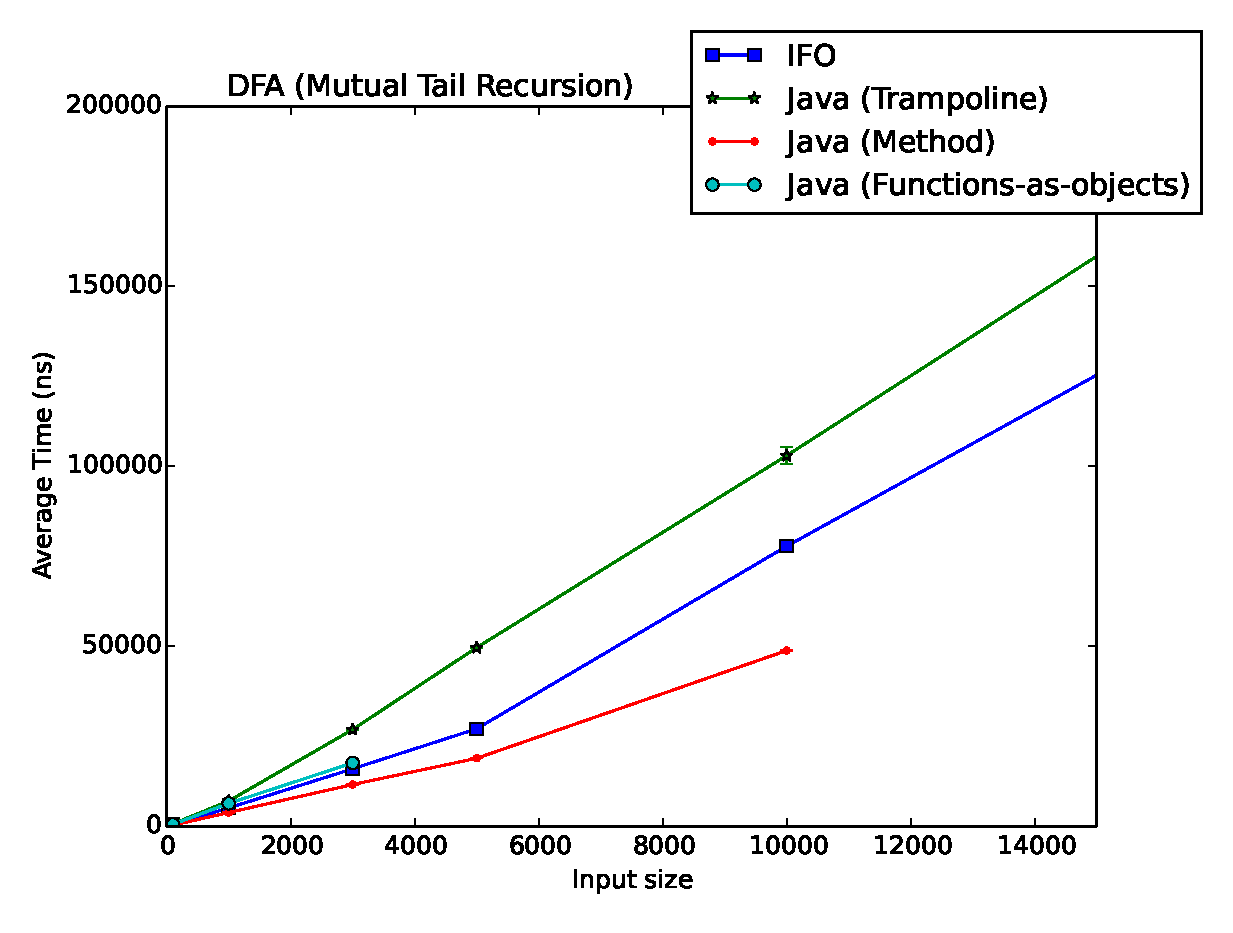
\includegraphics[width=8cm]{./src/img/dfa1.eps}}\end{minipage} &
\begin{minipage}{8cm}{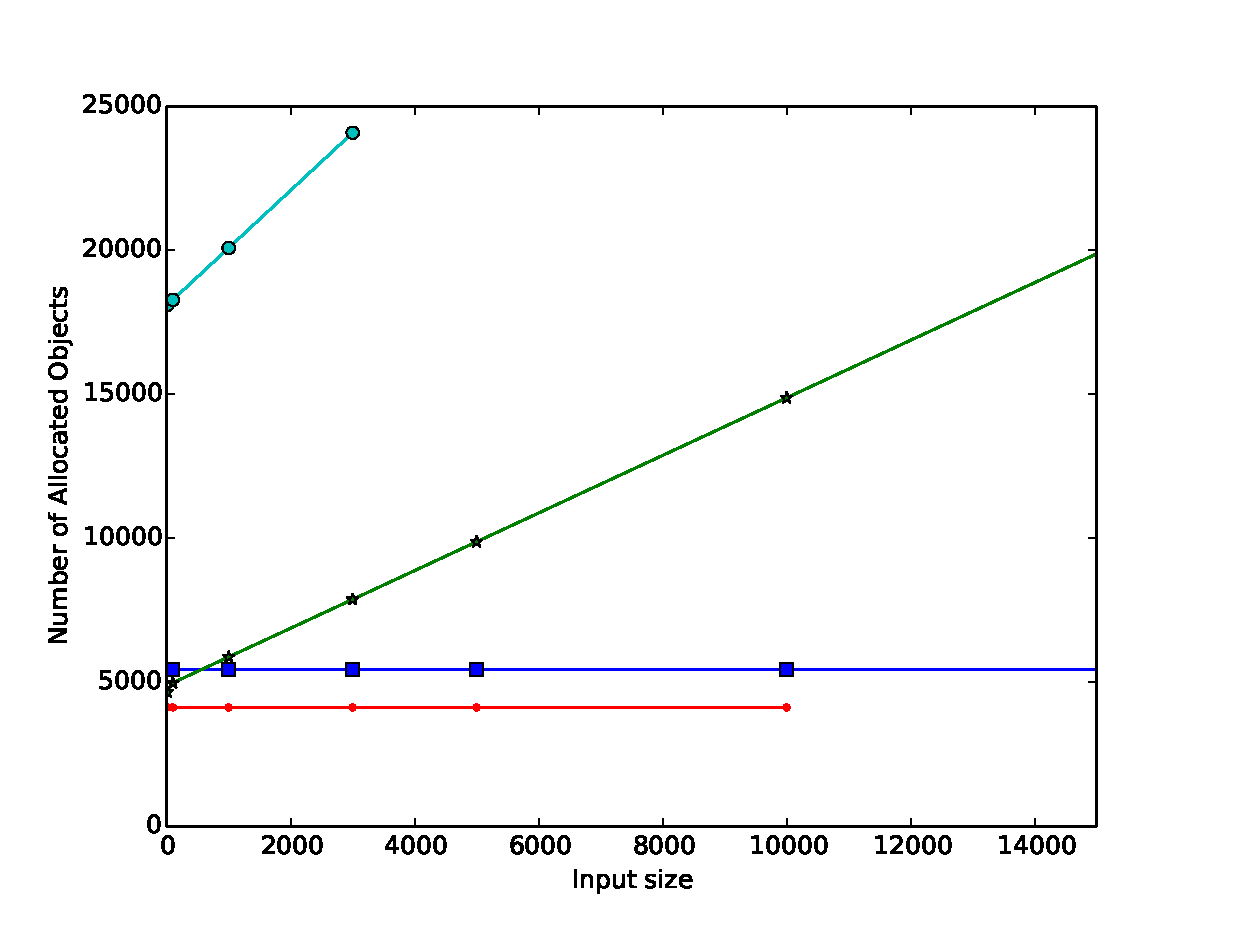
\includegraphics[width=8cm]{./src/img/dfa2.eps}}\end{minipage} 
\end{tabular}

\end{center}
\vspace{-15pt}
\caption{The DFA encoding: the reported times are averages of 10 measured runs and corresponding standard deviations; the last two columns show the minimum and maximum numbers of total allocated objects on heap from isolated profiled runs with all input lengths. Due to space limitations, the x-axes of plots are cropped at 15000 for clarity.}

\label{fig:dfa}
\end{figure*}

\begin{figure*}[h!t]
\vspace{5pt}
 \begin{center} 
\begin{tabular}{|l|l|l|l|l|l|}
\hline
\multicolumn{1}{|r|}{\textit{\textbf{Input length (time units)}}} & 10 ($\mu s$)  & 20 ($\mu s$)   & 40 ($ms$)     & 50 ($ms$)     & 75 ($ms$)     \\ \hline
\textbf{Java (Trampoline-based)}                                       & $17.10 \pm 0.26$ & $320.42 \pm 5.88$ & $14.84 \pm 0.27$ & $62.35 \pm 1.06$ & $1044.61 \pm 12.99$ \\ \hline
\textbf{IFO}                                                      & $11.06 \pm 0.55$ & $289.19 \pm 6.52$ & $12.70 \pm 0.26$ & $48.47 \pm 1.08$ & $805.06 \pm 7.06$ \\ \hline
\textit{Relative speedup}                                         & 54.6\%           & 10.8\%            & 16.9\%           & 28.6\%           & 29.8\%          \\ \hline
\end{tabular}
\end{center}

\vspace{-5pt}
\caption{The 0-1 Knapsack Problem encoded using CPS for different input sizes (the length of weight and value lists) for a fixed total weight of 10: the reported times are averages of 10 measured runs and corresponding standard deviations. 
%Method-based and FAO implementations could not run beyond the input of length 10; their execution times at 10 were $9.68 \pm 0.20~\mu s$ and $13.79 \pm 0.22~\mu s$ respectively.
}

\label{fig:cps}
\end{figure*}

\section{Evaluation}

%Apart from the correctness and uniformity of the representation, 
\name performs well in common FP scenarios. Our evaluation of this claim consists of two
parts. We first compare time performance results of benchmark programs
that isolate different call behaviors. Then, we demonstrate two
application use cases and examine their scalability.

\subsection{Isolated Call Behavior}\label{sec:micro}

In this experiment, we want to evaluate runtime performance of
programs representing different common call behaviors in FP.
We compare the measured average times of these programs
written in \name (to assess IFOs) and of corresponding
programs written in Scala, Clojure, and Java using standard functions
(as methods) and trampolines.

\paragraph{Benchmark Design.}
We wrote the benchmark programs in the extended System F for our
compilation process and in the following JVM-hosted languages in their
latest stable versions:

\begin{itemize}

  \item \emph{Scala} (2.11.2): Scala is one of the most popular
    strongly-typed multi-paradigm languages on the JVM
    \cite{Odersky2014b}. It directly compiles down to the Java
    bytecode and applies various optimizations. In order to encode
    mutually recursive tail calls, we used the provided trampoline
    facility (\texttt{scala.util.control.} \texttt{TailCalls}).

  \item \emph{Clojure} (1.6.0): Clojure is a dynamically-typed,
    functional language which compiles to the Java bytecode
    \cite{Hickey2008}. For mutually recursive tail calls, we used
    \texttt{tramp} from \texttt{clojure.core.} \texttt{logic}.
  
  \item \emph{Java} (1.8.0\_25): We implemented two versions, one
    version using method calls in Java 8 and one using custom
    (hand-written and optimized) trampolines.

\end{itemize}
  
\noindent To evaluate IFOs, we used the \name compiler with all the
optimizations mentioned in Sections \ref{sec:tce} and
\ref{sec:implementation}.

\noindent We executed all benchmarks on the following platform with
the latest Java HotSpot\texttrademark VM (1.8.0\_25):
Intel\textregistered Core\texttrademark i5 3570 CPU, 1600MHz DDR3 4GB
RAM, Ubuntu 14.04.1.
  
\noindent For the automation of performance measurement, we used the
Java Microbenchmark Harness (JMH) tool which is a part of OpenJDK
\cite{jmh}. Based on the provided annotations, JMH measures execution
of given programs. In addition to that, it takes necessary steps to
gain stable results. They include non-measured warm-up iterations for
JITC, forcing garbage collection before each benchmark, and running
benchmarks in isolated VM instances. We configured JMH for 10 warm-up
runs and 10 measured runs from which we compute averages.

\paragraph{Programs.}

We chose four programs to represent the following behaviors:

\begin{itemize}

  \item \emph{Non-tail recursive calls}: Computing the factorial and
    Fibonacci numbers using naive algorithms.

  \item \emph{Single method tail recursive calls}: Computing factorial
    using a tail recursive implementation.

  \item \emph{Mutually recursive tail calls}: Testing evenness and
    oddness using two mutually recursive functions.
\end{itemize}

\noindent Non-tail recursive programs present two examples of general
recursive calls and we executed them, altogether with the tail
recursive programs, on low input values (not causing
\lstinline{StackOverflow} exceptions in default JVM settings). In
addition to that, we executed the tail recursive programs on high input
values in which method-based implementations threw
\lstinline{StackOverflow} exceptions in default JVM settings.
  
\paragraph{Results.}

We show the results in Figure \ref{fig:micro}. Its left part shows
the result for low input values in IFOs, method implementations in all
the other languages and the fastest trampoline implementation (Java);
the plot is normalized to the Java method-based
implementation's results. The right part shows the result for high input values
in IFO- and trampoline-based implementations; the plot is normalized to results of 
IFO-based implementations.

For low input values, we can see that IFO-based implementations run
slightly slower than method-based ones. However, their overhead is
small compared with the fastest trampoline implementations in our
evaluation. IFOs ran 0.1 to 1.7-times slower than method-based
representations, whereas the fastest trampolines ran 7.7 to 22.3-times
slower. In the tail recursive programs, Scala ran slightly faster than
standard Java methods due to its compiler optimizations. Clojure has
an additional overhead, because its compiler enforces integer overflow
checking.

For the high input values, the method-based implementations threw a
\lstinline{StackOverflow} exception in default JVM settings, unlike
IFOs and trampoline implementations which can continue executing with
this input. IFOs ran 3.9 to 12.2-times faster (excluding Clojure) than
trampoline implementations. Again, Clojure suffered from its
additional overhead and threw an integer overflow exception in the
tail recursive factorial. Using BigIntegers would prevent this, but
we wanted to isolate the call behavior in this experiment, i.e. avoid
any extra overhead from other object allocations.

\subsection{Applications}

In this experiment, we examine the time and memory scalability of IFOs
and alternative closure representations (methods,
functions-as-objects, and trampolines) in two applications which
make use of tail calls. Unlike Section \ref{sec:micro}, where
the programs isolated costs of plain recursive calls, the applications
here represent a more realistic behavior with other costs, such as
non-recursive method calls, calls to other API methods or partial applications.

We implemented the applications in \name to assess
IFOs and in Java to assess different closure representations: method
calls, Java 8's lambdas (functions-as-objects), and custom
trampolines. We chose Java, because our custom implementation of
trampolines performed best in the isolated call behavior
experiments. Using plain Java implementations, we can examine the
runtime behavior of different representations without potential
compiler overheads.  We performed the time measurement in the same
setting as in the previous experiment. For the memory, we report the
total number of allocated objects on heap in the isolated application
runs, as measured by HPROF~ \cite{hprof}, the JDK's profiling tool.

\paragraph{DFA Encoding.}\label{sec:dfa}

One common idiom in functional programming is encoding finite states
as tail recursive functions and state transitions as mutual calls
among these functions. One trivial example of this is the naive
even-odd program which switches between two states. A more useful
application is in the implementation of finite state automata
\cite{Krishnamurthi2006}. Normally, functional language programmers
seek this idiom for its conciseness. However in JVM-hosted functional
languages, programmers tend to avoid this idiom, because they either
lose correctness (\lstinline{StackOverflow} exceptions in a
method-based representation) or performance (in a trampoline-based
one). In this experiment, we implemented a DFA recognizing a regular
expression $(AAB^{*}|A^{*}B)^{+}$ and measured the performance on
randomly generated Strings with different lengths.

We show the result of this experiment in Figure \ref{fig:dfa}. The
FAO-based implementation ran slowest out of all implementations and threw
\lstinline{StackOverflow} exception with a smaller input than the
method-based implementation. That is because it creates extra objects
and performs extra calls due to its representation. As in the isolated
calls experiment, the IFO-based implementation ran about 0.5-times slower than method-based
implementation. Trampolines, however, ran about 2-times slower. The IFO-
and trampoline-based implementations continued executing after method-based
one threw a \lstinline{StackOverflow} exception. The IFO-based
implementation was about 0.2-times faster than the trampoline one for 
larger inputs.

What is more important here is the memory consumption. IFOs, similarly
to the method-based implementation, allocated a constant number of
objects on heap. The trampoline one, however, increased its object
allocation with the input, because it needed to create an object for 
each tail call.

\paragraph{CPS Encoding of Knapsack.}\label{sec:cps}

Tail calls find their application in continuation-passing style
\cite{Steele1975} where each call is a tail call.  In this
application, we encoded a naive implementation of the 0-1 Knapsack
Problem with multiple recursive calls and also non-recursive tail
calls.  In the experiment, we fixed the total weight to 10 and
generated input values and weights lists of different sizes: we
generated weights as consecutive sequences 1 to 5 and values as
$i\times weight[i]$.

We show the results in Figure \ref{fig:cps}. This implementation contains 
partial applications and a pure method-based implementation is impossible in this style.
The method- and FAO-based implementations could not run beyond the input of length 10 due to a \lstinline{StackOverflow} exception; their execution times at 10 were $9.68 \pm 0.20~\mu s$ and $13.79 \pm 0.22~\mu s$ respectively. IFOs ran 10.8\% to 54.6\% faster than the trampoline implementation in different input lengths.

\subsection{Discussion}

The programs benchmarked in Section \ref{sec:micro} stressed the time
spent on recursive calls. These programs are quite simple, but
representative of common patterns of functional programming. IFOs gave
a 3.9 to 12.2-times speed-up over the trampoline implementations. This
huge gain is also due to other optimizations in our compiler. In
particular, since those programs have small and simple definitions,
inlining is beneficial and gives a big performance gain on top of the
gains for TCE. In the more complex scenarios of Section
\ref{sec:dfa}, the tail calls are not the only runtime cost, so the
overhead of trampolines is much smaller. Still, IFO programs gained a
speed-up of 0.1 to 0.5 over our hand-written and optimized
trampolines.  The other benefit for programs with tail recursion
is the constant memory overhead of calls in IFOs.
This also appears in method-based implementations, but they
throw a \lstinline{StackOverflow} exception in larger inputs and IFOs
do not.

